\documentclass[10pt,a4paper]{article}
\usepackage[margin=19mm]{geometry}
\usepackage{booktabs,longtable,graphicx}
\usepackage[T1]{fontenc}
\usepackage{lmodern}
\usepackage[colorlinks=true,linkcolor=blue]{hyperref}
\setlength{\parskip}{5pt}
\begin{document}
\begin{center}\LARGE\bfseries T3 reduced-scalar numerical benchmarks\end{center}
\noindent\textbf{Scope:} 16 representations, two frozen-UV scenarios; additional scalar couplings initially zero. Historical UV-running inputs are examined as exploratory RGE diagnostics.\\
\textbf{Acceptance:} Five-observable Gaussianised NuFIT $\chi^2\leq 5.86$. Individual fits: 32/32. Unchanged scenario-specific A(-2) Yukawas: 10/32.
\section*{Frozen-UV Yukawa comparisons}
\small\begin{longtable}{lrrrr}
\toprule Model & Low ind. $\chi^2$ & Low A(-2) $\chi^2$ & High ind. $\chi^2$ & High A(-2) $\chi^2$ \\
\midrule\endfirsthead
\toprule Model & Low ind. $\chi^2$ & Low A(-2) $\chi^2$ & High ind. $\chi^2$ & High A(-2) $\chi^2$ \\
\midrule\endhead
A\_+0 & 1.12149e-11 & 0.00817089 & 0.00516295 & 0.00758579 \\
A\_-2 & 5.30105e-17 & 5.30105e-17 & 3.53986e-11 & 3.53986e-11 \\
A\_-4 & 2.08195e-16 & 11527.7 & 2.86028e-14 & 11464.1 \\
B\_+1 & 1.1989e-21 & 1.4739 & 3.44636e-11 & 2.1874 \\
B\_-1 & 8.93793e-18 & 37.3954 & 1.06771e-08 & 35.4519 \\
B\_-3 & 8.29795e-15 & 12177.8 & 1.48272e-09 & 12124.1 \\
C\_+1 & 6.60223e-20 & 9273.32 & 3.48456e-20 & 9256.32 \\
C\_-1 & 2.28605e-10 & 9749.82 & 2.45329e-18 & 9739.22 \\
C\_-3 & 8.04078e-11 & 17818.8 & 8.57308e-15 & 17797.4 \\
D\_+0 & 2.57559e-12 & 0.000202375 & 1.04657e-08 & 0.000209023 \\
D\_+2 & 4.12536e-12 & 232.824 & 8.5912e-11 & 238.68 \\
D\_-2 & 1.2035e-10 & 0.0128843 & 3.4551e-11 & 0.0122503 \\
E\_+0 & 1.36835e-09 & 3922.1 & 4.12798e-11 & 4106.15 \\
E\_+2 & 2.43592e-17 & 2932.51 & 5.58612e-11 & 3106.76 \\
E\_-2 & 1.18552e-09 & 3915.55 & 3.02698e-15 & 4099.54 \\
E\_-4 & 8.27006e-12 & 15394.6 & 8.65198e-11 & 15437.3 \\
\bottomrule\end{longtable}\normalsize
\noindent Class E uses $\lambda_{T3}=2.5\times10^{-9}$ (low) and $0.25$ (high); classes A--D use $5\times10^{-9}$ and $0.5$.
\section*{Exploratory fixed-input UV-running diagnostic}
\noindent The nominal 1 TeV scalar-EFT endpoints below are \emph{formal diagnostics}, not rematched threshold masses. No historical seed satisfies the original 0.5--5 TeV scalar window.
\small\begin{longtable}{lrrr}
\toprule Model & Formal $m_{S_1}$ [TeV] & Formal $m_{S_2}$ [TeV] & $\rho_F$ \\
\midrule\endfirsthead
\toprule Model & Formal $m_{S_1}$ [TeV] & Formal $m_{S_2}$ [TeV] & $\rho_F$ \\
\midrule\endhead
A\_+0 & 40.9155 & 42.3856 & 0.411017 \\
A\_-2 & 39.89 & 40.5393 & 0.380523 \\
A\_-4 & 35.1197 & 59.4371 & 0.524996 \\
B\_+1 & 30.4184 & 37.8432 & 0.35929 \\
B\_-1 & 72.8071 & 100.076 & 1.07037 \\
B\_-3 & 31.3093 & 36.4894 & 0.356154 \\
C\_+1 & 63.5017 & 66.1264 & 0.586791 \\
C\_-1 & 118.583 & 169.101 & 1.69761 \\
C\_-3 & 63.5579 & 65.0881 & 0.590349 \\
D\_+0 & 34.1921 & 51.7206 & 0.495521 \\
D\_+2 & 45.4834 & 46.3077 & 0.407491 \\
D\_-2 & 34.7952 & 50.8104 & 0.492456 \\
E\_+0 & 46.442 & 64.0919 & 0.644065 \\
E\_+2 & 43.4201 & 44.4576 & 0.372919 \\
E\_-2 & 45.304 & 56.5035 & 0.525467 \\
E\_-4 & 45.7779 & 62.6794 & 0.530942 \\
\bottomrule\end{longtable}\normalsize
\section*{Interpretation and limitations}
\begin{itemize}
\item Independent Yukawa fits are flexible: 18 real Yukawa parameters are fitted to five oscillation observables, so a small $\chi^2$ is not an independent prediction.
\item The zero-extra-scalar-coupling boundary is a restricted leading-order approximation, not the complete scalar potential.
\item Additional B/C quartics generated by one-loop RGEs are not inserted into the leading fixed-order $C_5$ coefficient.
\item Four extreme-hypercharge models use nonuniform legacy $C_5$ sources. Full Matchete/RGBeta normalisation and general sequential Wilson matching have not been certified.
\item Heavy scalar diagnostics from running UV do not justify using the nominal 1 TeV scalar matching as a physical threshold.
\end{itemize}
\clearpage
\begin{figure}[p]\centering
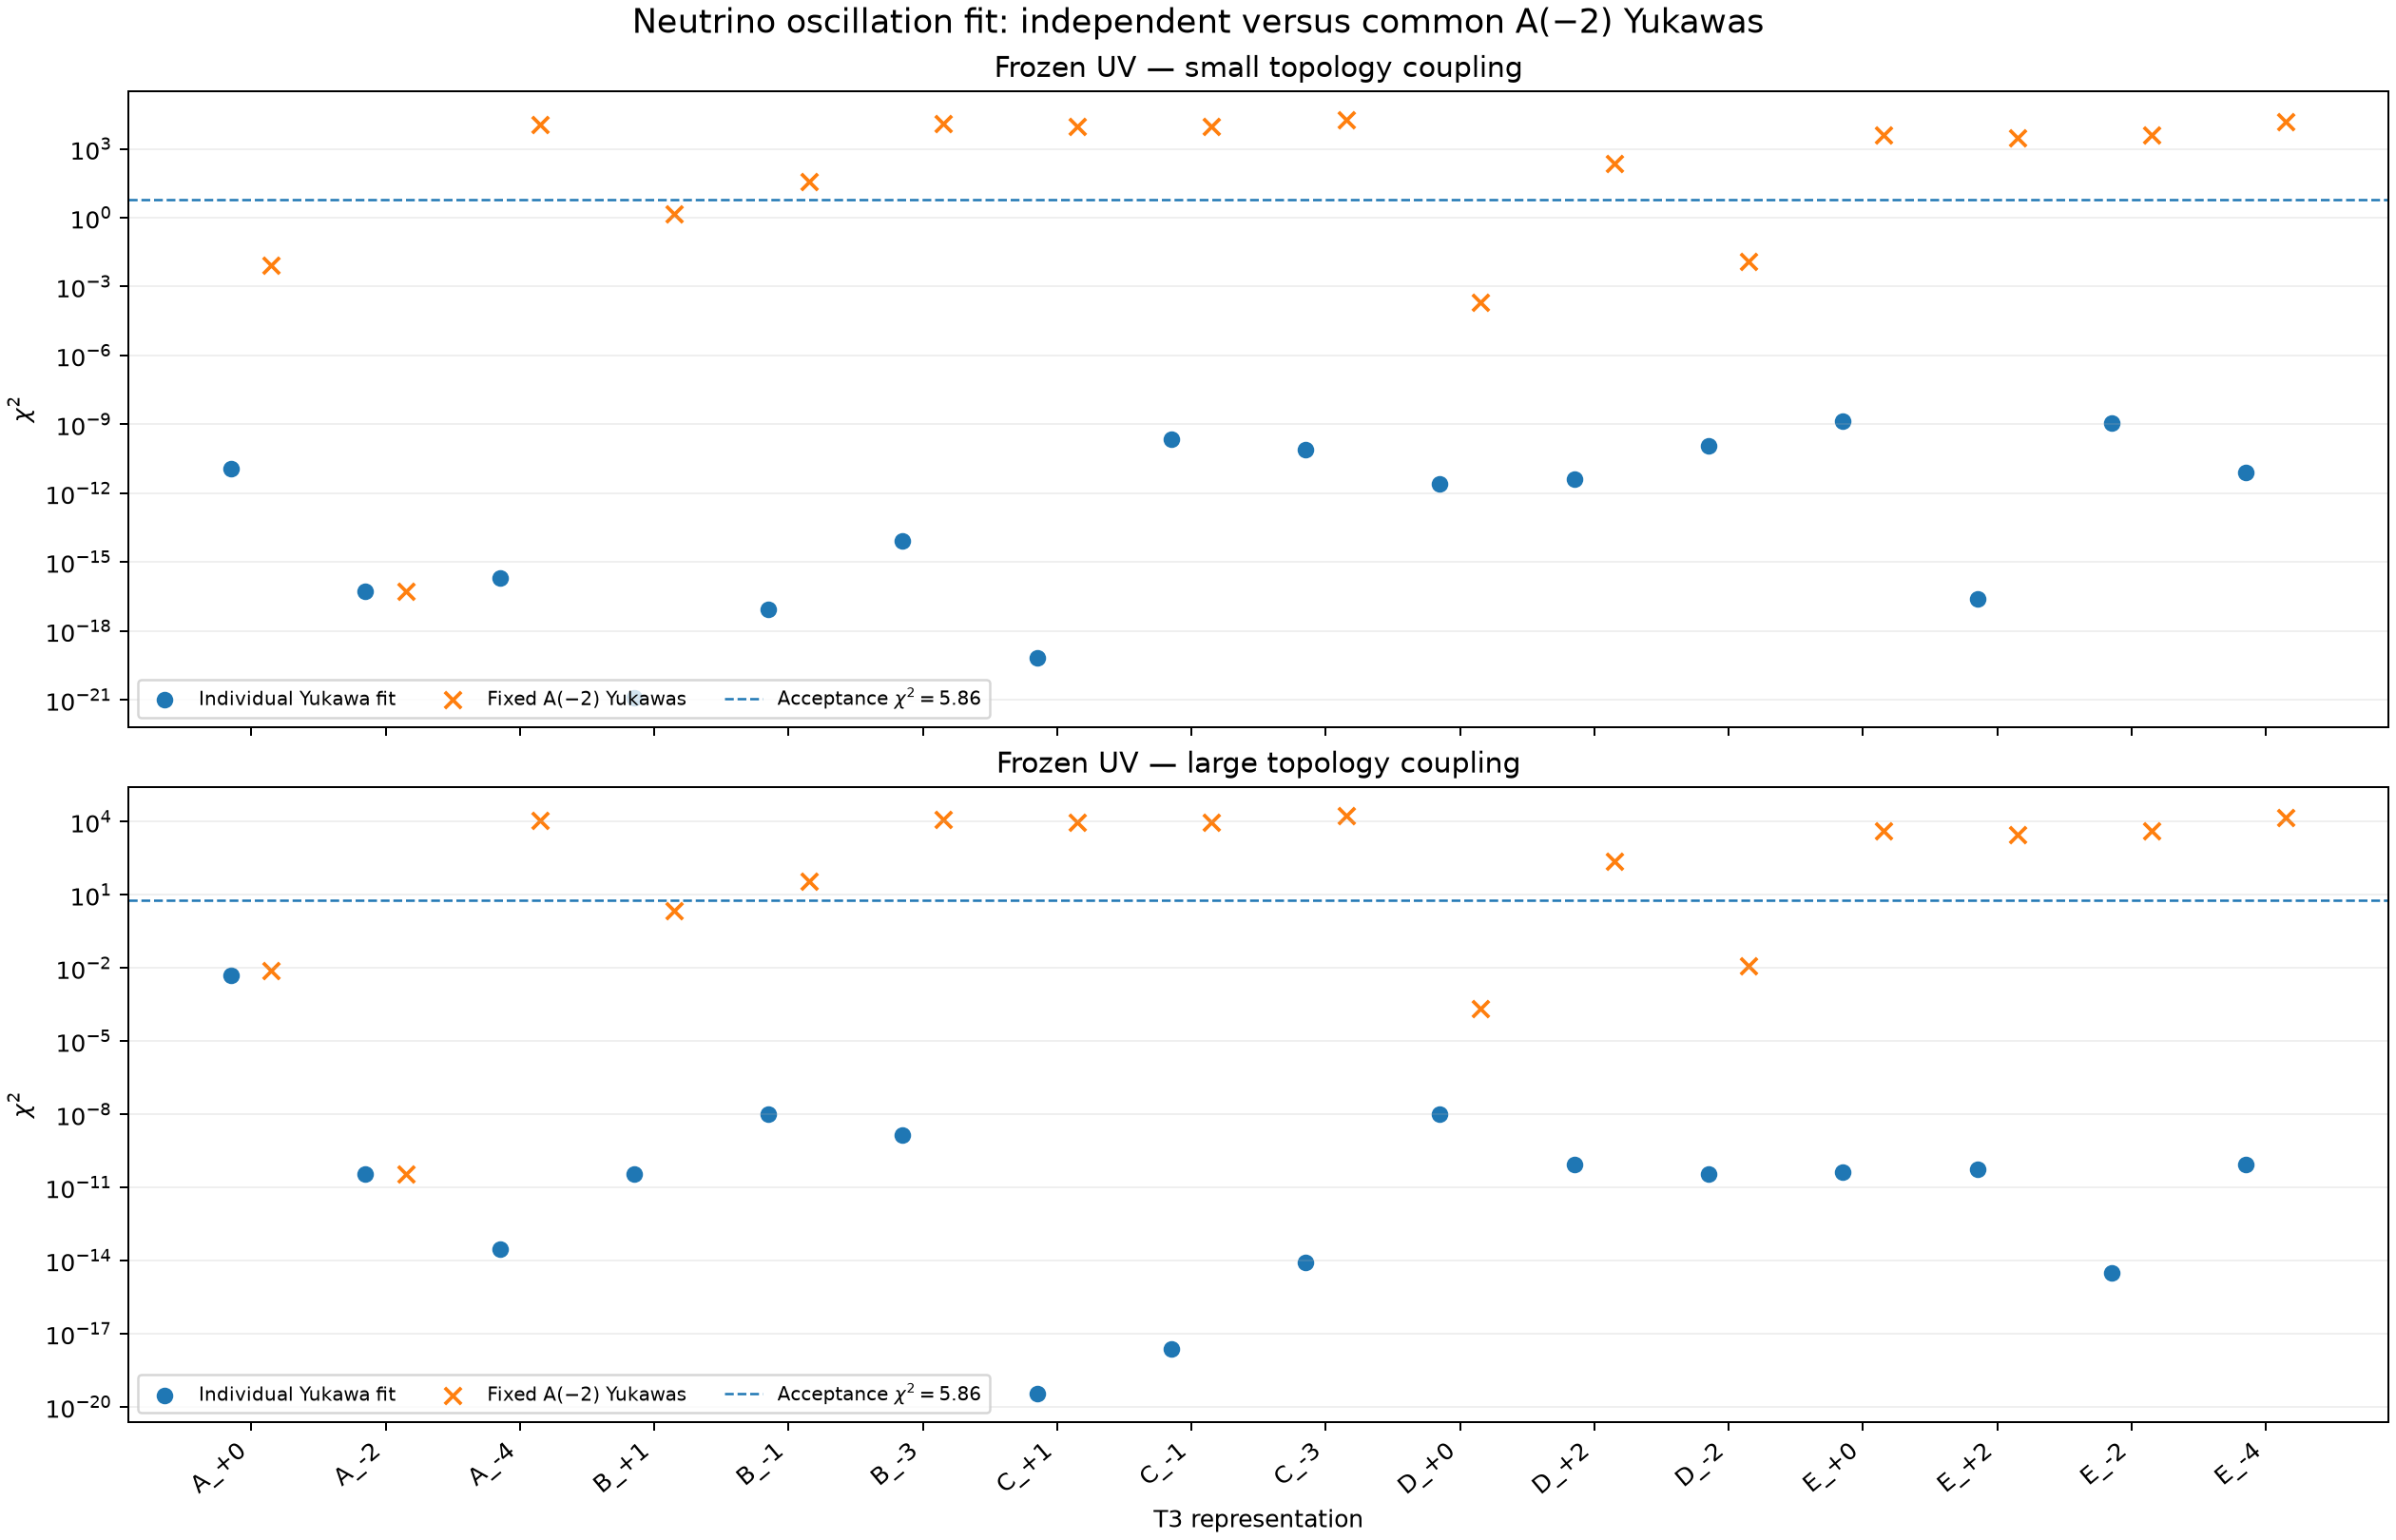
\includegraphics[width=\textwidth,height=0.78\textheight,keepaspectratio]{assets/frozen_chi2_comparison.png}
\caption{Frozen-UV independent versus shared fits}
\end{figure}
\clearpage
\clearpage
\begin{figure}[p]\centering
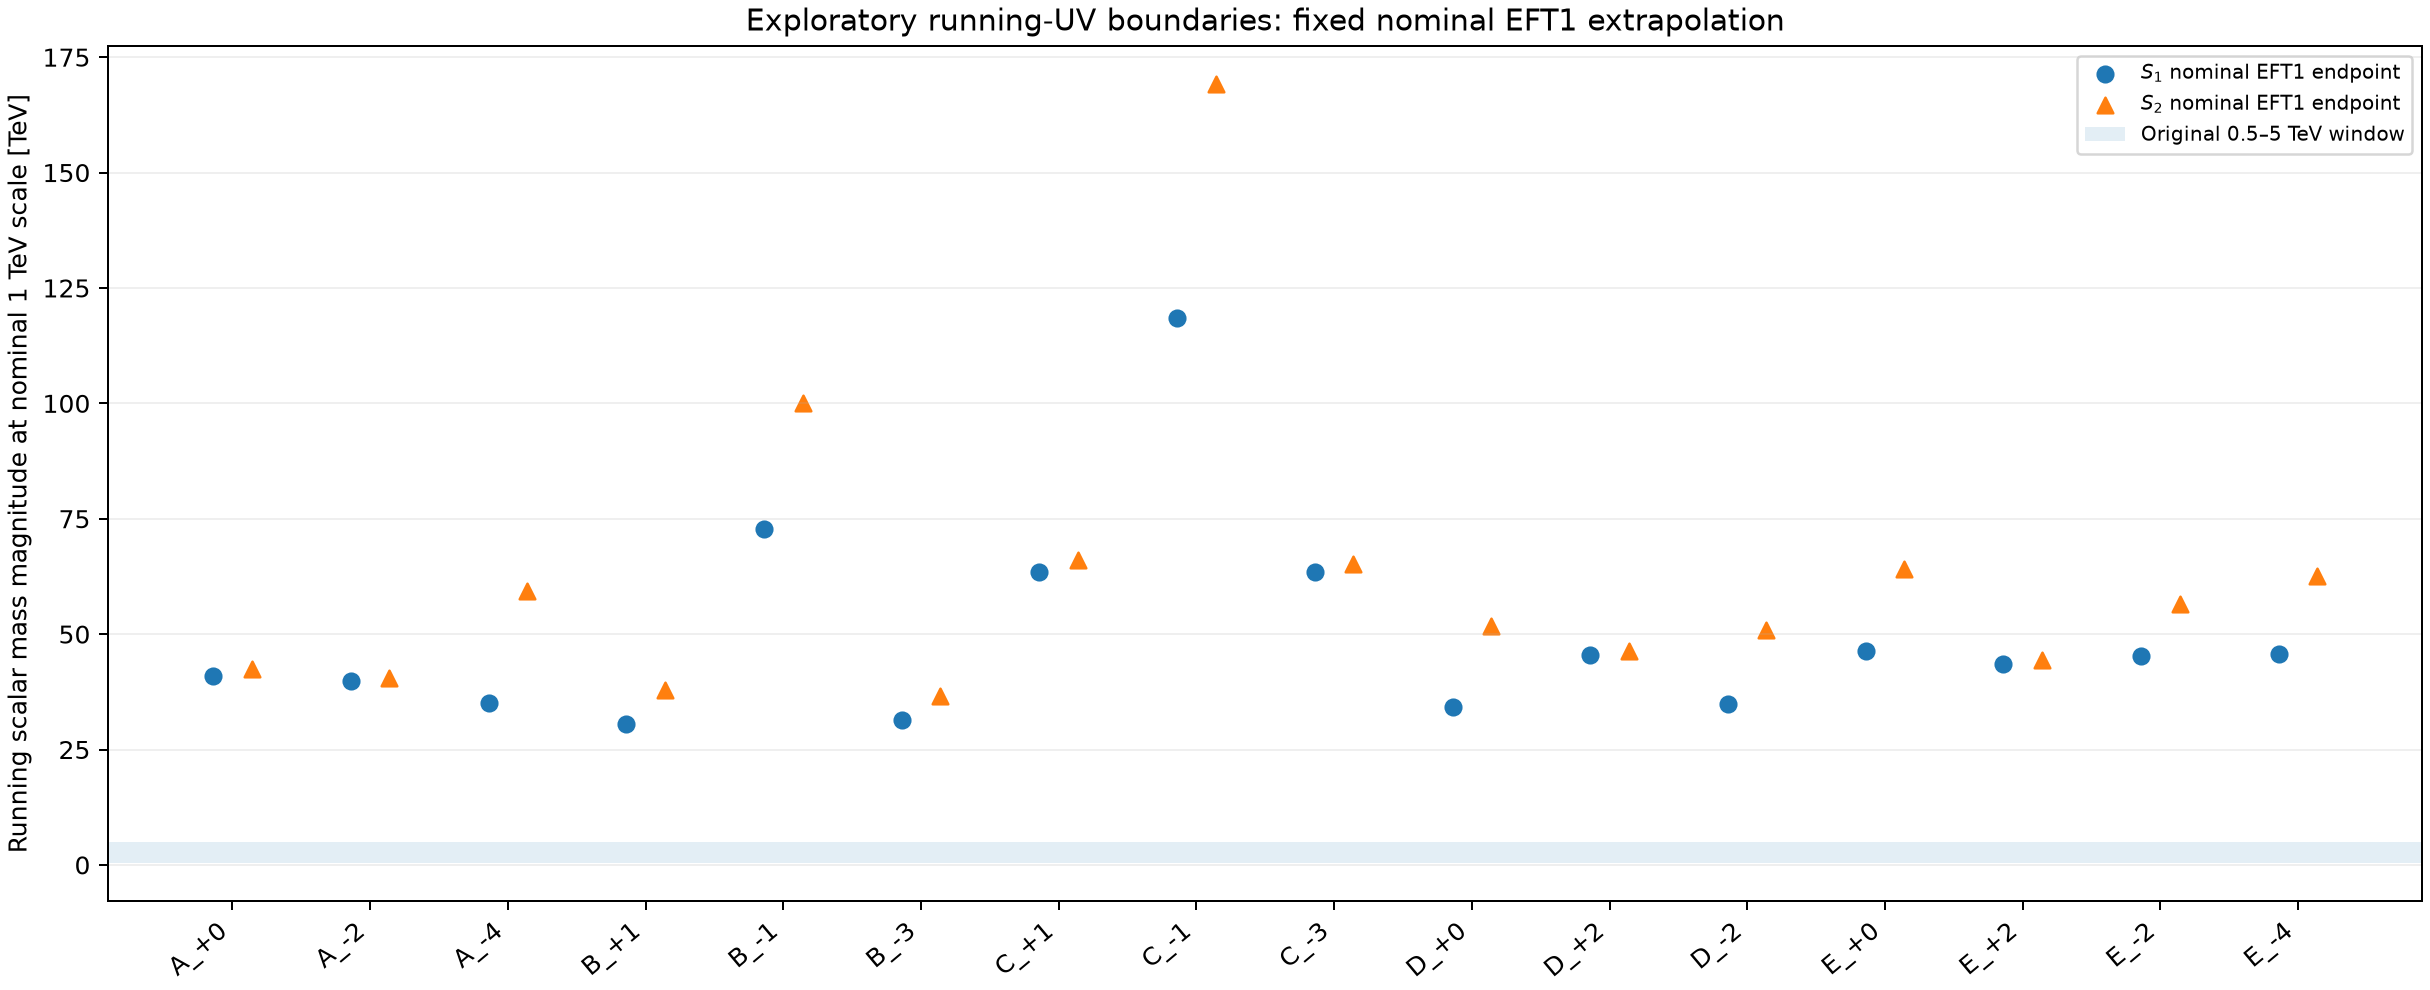
\includegraphics[width=\textwidth,height=0.78\textheight,keepaspectratio]{assets/running_uv_formal_mass_endpoints.png}
\caption{Formal scalar masses at nominal 1 TeV}
\end{figure}
\clearpage
\clearpage
\begin{figure}[p]\centering
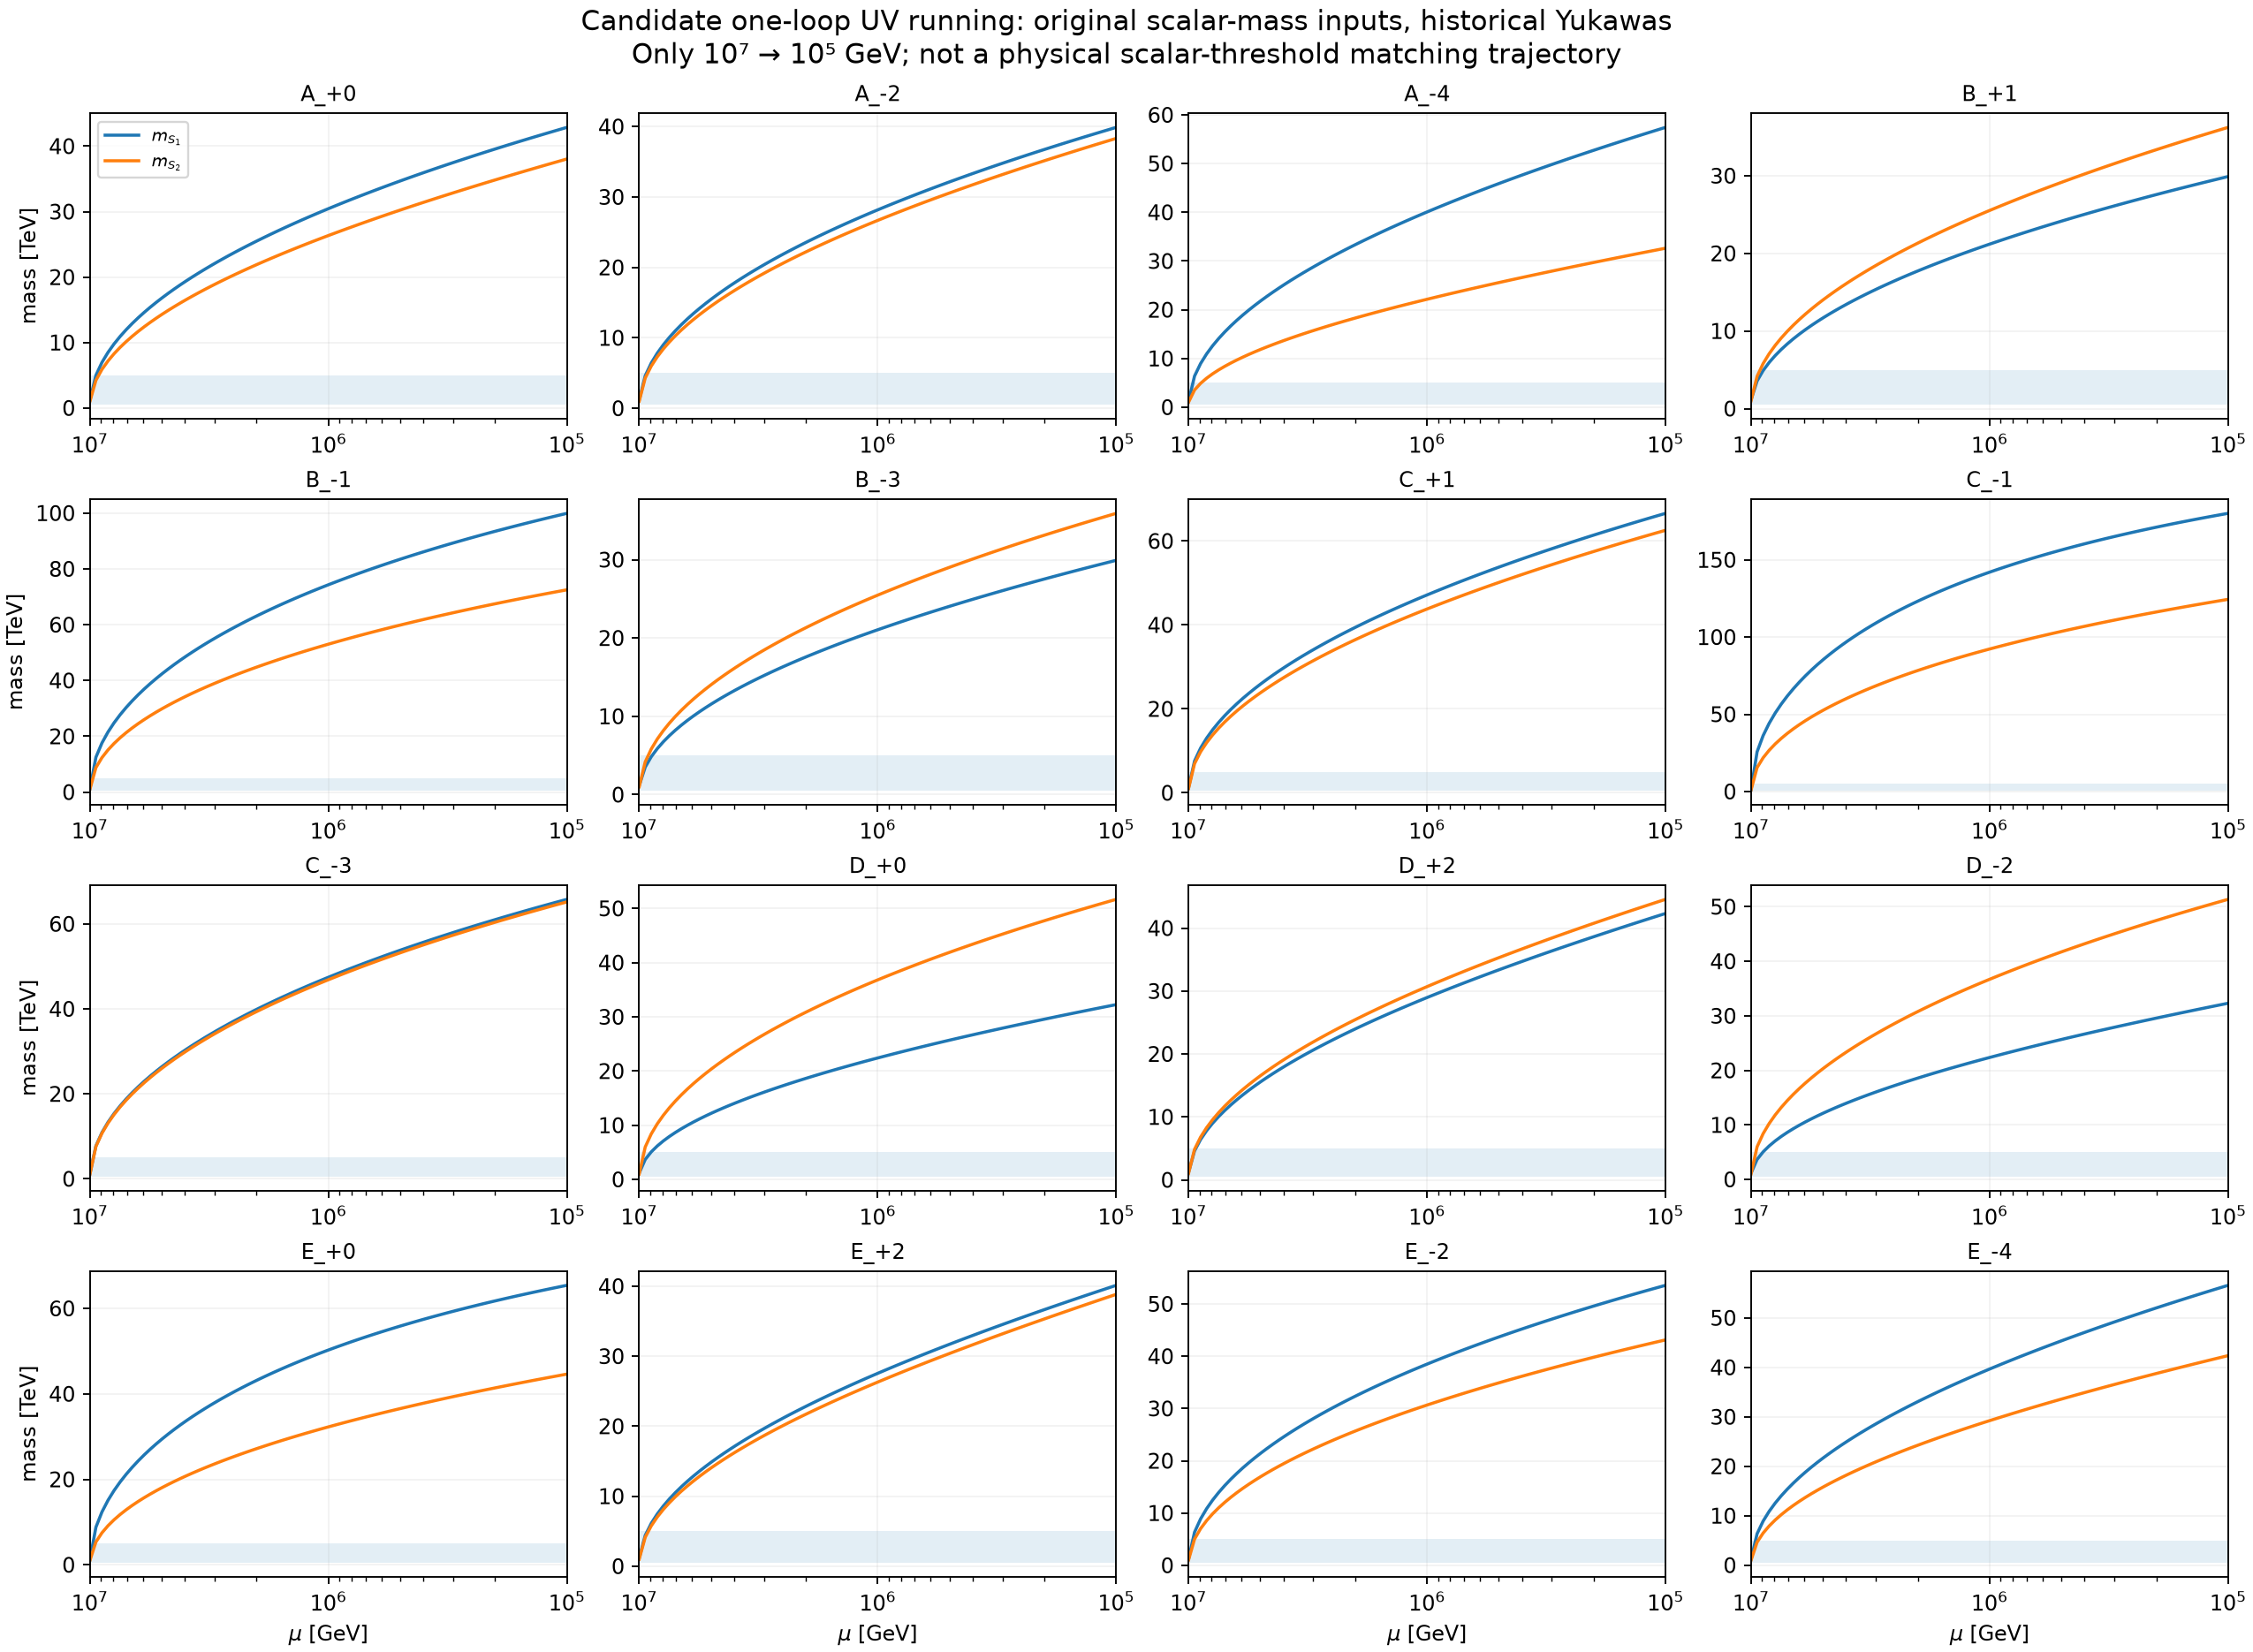
\includegraphics[width=\textwidth,height=0.78\textheight,keepaspectratio]{assets/running_uv_scalar_trajectories.png}
\caption{UV-running scalar trajectories, 10$^7$--10$^5$ GeV}
\end{figure}
\clearpage
\end{document}
